\documentclass[11pt]{article}

% Change "review" to "final" to generate the final (sometimes called camera-ready) version.
% Change to "preprint" to generate a non-anonymous version with page numbers.
\usepackage[review]{acl}

% Standard package includes
\usepackage{times}
\usepackage{latexsym}

% For proper rendering and hyphenation of words containing Latin characters (including in bib files)
\usepackage[T1]{fontenc}
% For Vietnamese characters
% \usepackage[T5]{fontenc}
% See https://www.latex-project.org/help/documentation/encguide.pdf for other character sets

% This assumes your files are encoded as UTF8
\usepackage[utf8]{inputenc}

% This is not strictly necessary, and may be commented out,
% but it will improve the layout of the manuscript,
% and will typically save some space.
\usepackage{microtype}

% This is also not strictly necessary, and may be commented out.
% However, it will improve the aesthetics of text in
% the typewriter font.
\usepackage{inconsolata}

%Including images in your LaTeX document requires adding
%additional package(s)
\usepackage{graphicx}

% If the title and author information does not fit in the area allocated, uncomment the following
%
%\setlength\titlebox{<dim>}
%
% and set <dim> to something 5cm or larger.

\title{Evaluating Adaptive Step Size Strategies in Convex Quadratic Optimization}

% Author information can be set in various styles:
% For several authors from the same institution:
% \author{Author 1 \and ... \and Author n \\
%         Address line \\ ... \\ Address line}
% if the names do not fit well on one line use
%         Author 1 \\ {\bf Author 2} \\ ... \\ {\bf Author n} \\
% For authors from different institutions:
% \author{Author 1 \\ Address line \\  ... \\ Address line
%         \And  ... \And
%         Author n \\ Address line \\ ... \\ Address line}
% To start a separate ``row'' of authors use \AND, as in
% \author{Author 1 \\ Address line \\  ... \\ Address line
%         \AND
%         Author 2 \\ Address line \\ ... \\ Address line \And
%         Author 3 \\ Address line \\ ... \\ Address line}

\author{First Author \\
  Affiliation / Address line 1 \\
  Affiliation / Address line 2 \\
  Affiliation / Address line 3 \\
  \texttt{email@domain} \\\And
  Second Author \\
  Affiliation / Address line 1 \\
  Affiliation / Address line 2 \\
  Affiliation / Address line 3 \\
  \texttt{email@domain} \\}

%\author{
%  \textbf{First Author\textsuperscript{1}},
%  \textbf{Second Author\textsuperscript{1,2}},
%  \textbf{Third T. Author\textsuperscript{1}},
%  \textbf{Fourth Author\textsuperscript{1}},
%\\
%  \textbf{Fifth Author\textsuperscript{1,2}},
%  \textbf{Sixth Author\textsuperscript{1}},
%  \textbf{Seventh Author\textsuperscript{1}},
%  \textbf{Eighth Author \textsuperscript{1,2,3,4}},
%\\
%  \textbf{Ninth Author\textsuperscript{1}},
%  \textbf{Tenth Author\textsuperscript{1}},
%  \textbf{Eleventh E. Author\textsuperscript{1,2,3,4,5}},
%  \textbf{Twelfth Author\textsuperscript{1}},
%\\
%  \textbf{Thirteenth Author\textsuperscript{3}},
%  \textbf{Fourteenth F. Author\textsuperscript{2,4}},
%  \textbf{Fifteenth Author\textsuperscript{1}},
%  \textbf{Sixteenth Author\textsuperscript{1}},
%\\
%  \textbf{Seventeenth S. Author\textsuperscript{4,5}},
%  \textbf{Eighteenth Author\textsuperscript{3,4}},
%  \textbf{Nineteenth N. Author\textsuperscript{2,5}},
%  \textbf{Twentieth Author\textsuperscript{1}}
%\\
%\\
%  \textsuperscript{1}Affiliation 1,
%  \textsuperscript{2}Affiliation 2,
%  \textsuperscript{3}Affiliation 3,
%  \textsuperscript{4}Affiliation 4,
%  \textsuperscript{5}Affiliation 5
%\\
%  \small{
%    \textbf{Correspondence:} \href{mailto:email@domain}{email@domain}
%  }
%}

\begin{document}
\maketitle
\begin{abstract}
In this paper, we tackle the challenge of evaluating and benchmarking various adaptive step size strategies specifically within the realm of convex quadratic optimization problems. This work is highly relevant as adaptive step size strategies are pivotal in optimization for effectively tackling problems with diverse difficulty levels, and convex quadratic functions often serve as a fundamental proxy for more complex optimization scenarios. The difficulty lies in selecting a comprehensive set of adaptive step size strategies, ensuring fair and thorough testing, and accurately measuring their performance while balancing computational efficiency with accuracy. Although adaptive step size strategies have been a topic of extensive study, their specific application and benchmarking against convex quadratic functions have not been exhaustively explored, presenting a novel contribution of this study. We address this gap by focusing on a targeted evaluation of existing strategies, using a set of synthetic convex quadratic functions generated from random symmetric positive definite matrices to ensure a diversity of condition numbers. We assess strategies including Gradient Descent with Armijo rule, Nesterov's Accelerated Gradient, Newton's Method with line search, and RMSProp, using metrics such as convergence rate, final solution accuracy, and computational cost. Our experiments reveal which strategies excel in terms of convergence speed and accuracy, providing valuable insights for algorithm selection in practical applications.
\end{abstract}


\section{Introduction}

Optimization is a cornerstone of numerous scientific and industrial applications, where adaptive step size strategies enhance algorithmic efficiency. These strategies are crucial within the realm of convex quadratic optimization, a fundamental class of problems that frequently acts as a proxy for more complex scenarios . Convex quadratic functions, with their well-defined curvature, provide a simplified yet robust framework for evaluating optimization techniques. This paper endeavors to evaluate and benchmark various adaptive step size strategies in this context, emphasizing their convergence speed and accuracy.

Evaluating adaptive step size strategies is inherently challenging. It involves selecting a diverse set of strategies, ensuring fair and comprehensive testing, and accurately measuring performance \cite{Robles-Kelly2019IncorporatingTB}. The complexity is compounded by the need to balance computational efficiency with result accuracy. The right strategy choice can significantly impact the efficiency of solving an optimization problem, underscoring the importance of this research for both theoretical exploration and practical applications \cite{Tovbis2024NewtonianPO}.

While adaptive step size strategies have been widely studied, there is a gap in their specific application and benchmarking against convex quadratic functions. This study addresses this gap by conducting a comprehensive evaluation of existing strategies, including Gradient Descent with Armijo rule, Nesterov's Accelerated Gradient, Newton's Method with line search, and RMSProp. Our goal is to provide insights into the relative performance of these strategies regarding convergence rate, final solution accuracy, and computational cost.

The experiments utilize synthetic convex quadratic functions generated using random symmetric positive definite matrices, offering a range of condition numbers to test robustness. The effectiveness of each method is assessed by measuring convergence rate, accuracy of the final solution, and computational cost, offering a holistic view of each strategy's efficacy. Our contributions include:

- A detailed analysis of adaptive step size strategies in convex quadratic optimization.
- Insights into the strengths and limitations of each strategy.
- Guidance for selecting optimization algorithms in practical applications.
- Foundations for future research in more complex problem domains.

\section{Related Work}

In recent years, several methodologies have been developed to address optimization challenges with varying assumptions and techniques. Our research, motivated by the need to evaluate adaptive step size methods in the context of synthetic convex quadratic functions, shares some common ground with existing literature, yet also diverges in key aspects.

One notable approach is the use of delay-adaptive step-sizes for asynchronous learning \cite{Wu2022DelayadaptiveSF}, which focuses on adapting step sizes based on the delay in asynchronous settings. While this method is tailored to environments with communication delays, our study assumes synchronous updates, thus making direct application of their approach less relevant in our settings. Nonetheless, the concept of adaptive step-sizing is a parallel interest, and their methodology could provide insights into future extensions of our work to asynchronous contexts.

The work on Advances in Low-Memory Subgradient Optimization \cite{Dvurechensky2019AdvancesIL} addresses memory constraints in optimization processes. While our focus is not explicitly on memory efficiency, the low-memory techniques proposed could complement our study by reducing computational overhead in high-dimensional settings. However, the primary distinction lies in our exploration of convergence rates and accuracy, rather than memory efficiency.

In the realm of convex optimization, the study on On Low-Rank Convex-Convex Quadratic Fractional Programming  explores optimization within a specific class of problems using fractional programming. Our research does not delve into fractional programming; instead, we consider a broader class of convex quadratic problems with varying condition numbers. Thus, while both studies share an interest in quadratic functions, the methodological focus and application domains differ significantly.

The quantum search method for quadratic and multidimensional knapsack problems  presents an innovative approach using quantum computing techniques. While groundbreaking, this quantum-centric method diverges from our classical computational approach. As our study focuses on classical adaptive step size methods, a direct comparison is not feasible, although the exploration of quantum methods could be an intriguing future direction.

Adaptive Subgradient Methods for Online Learning and Stochastic Optimization \cite{Duchi2011AdaptiveSM} and Methods for Convex \((L_0,L_1)\)-Smooth Optimization: Clipping, Acceleration, and Adaptivity  both explore adaptive methodologies in optimization. These studies highlight the adaptability of subgradient methods in online and stochastic settings, offering parallels to our exploration of adaptive step sizes in deterministic environments. The primary contrast lies in the stochastic versus deterministic problem settings, necessitating distinct evaluation metrics and assumptions, but both share a fundamental interest in optimization efficiency.

Furthermore, the investigation into Optimizing \((L_0, L_1)\)-Smooth Functions by Gradient Methods \cite{Vankov2024OptimizingL} is relevant to our study, as it involves gradient-based methods for smooth functions. The methodologies proposed in this work could be leveraged as a comparative baseline in our experiments due to their focus on smooth function optimization, aligning with our interest in convergence and solution accuracy.

Finally, the study on Accelerated Sparse Recovery via Gradient Descent with Nonlinear Conjugate Gradient Momentum \cite{Hu2022AcceleratedSR} and On Low Complexity Acceleration Techniques for Randomized Optimization \cite{Stich2014OnLC} both contribute valuable insights into acceleration techniques for optimization. While our study emphasizes adaptive step sizing, the acceleration techniques discussed could be integrated into future iterations of our methods to enhance convergence rates.

In summary, while our research shares thematic connections with existing literature, it stands apart in its specific focus on adaptive step size methods applied to synthetic convex quadratic functions. Each of the discussed works provides complementary insights or methodologies that could inform future extensions of our study, though direct comparisons are not always feasible due to differing assumptions and methodological focuses.

\section{Method}

In this study, we aim to evaluate and benchmark various adaptive step size strategies specifically within the context of convex quadratic optimization problems. This section outlines the methodology employed to conduct this research, detailing the problem setup, the adaptive step size strategies considered, and the experimental protocol for assessing their performance.

\subsection{Synthetic Convex Quadratic Functions}

The core of our experimental setup is the generation of synthetic convex quadratic functions. This is achieved by constructing random symmetric positive definite matrices, ensuring a variety of condition numbers to test the robustness of the optimization strategies. Specifically, for each instance:

1. We generate a random matrix \( A \) of size \( n \times n \), where \( n \) is set to 100 for our experiments. This matrix is made symmetric and positive definite by computing the product \( A = A^T A \), thus ensuring the convexity of the quadratic function.
2. A random vector \( b \) is generated, also of size \( n \).
3. The objective function is then defined as \( f(x) = \frac{1}{2} x^T A x - b^T x \), where \( x \) is the variable to be optimized.

This setup allows us to simulate a range of convex quadratic problems with varying levels of difficulty, controlled by the condition number of the matrix \( A \).

\subsection{Adaptive Step Size Strategies}

We evaluated four distinct adaptive step size strategies, each chosen for their unique approach to handling convergence in optimization problems:

1. **Gradient Descent with Armijo Rule**: This strategy employs a backtracking line search method to adaptively choose the step size, ensuring a sufficient decrease in the objective function. The algorithm iteratively adjusts the step size based on the Armijo condition, using parameters such as \( \beta = 0.5 \) and \( \sigma = 1 \times 10^{-4} \). This ensures efficient convergence by adapting to the local curvature of the function .

2. **Nesterov's Accelerated Gradient (NAG)**: NAG is an enhancement of the basic gradient descent method, introducing an additional momentum term to accelerate convergence. The momentum parameter \( \alpha \) is set to 0.9, providing a balance between stability and speed \cite{Beck2009AFI}.

3. **Newton's Method with Line Search**: This method leverages the second-order derivative (Hessian) information to make more informed updates. The Hessian is constant and equal to \( A \) in this context. The line search ensures that each iteration makes significant progress toward the minimum \cite{Pei2014ATA}.

4. **RMSProp**: This stochastic optimization method adapts the learning rate by maintaining a moving average of squared gradients. It utilizes a decay rate of 0.9 and a small constant \( \epsilon = 1 \times 10^{-8} \) to ensure numerical stability .

\subsection{Experimental Protocol}

The experiments are structured to measure three key metrics for each optimization strategy:

- **Convergence Rate**: The number of iterations required for the algorithm to reach a defined tolerance level (\( 1 \times 10^{-6} \)) in terms of gradient norm.
- **Final Solution Accuracy**: The Euclidean distance between the obtained solution and the actual solution, providing a measure of how close the algorithm gets to the true minimum.
- **Computational Cost**: The time taken for each algorithm to converge, offering insight into the efficiency of the strategy.

Each algorithm is initialized with the same starting point \( x_0 = \mathbf{0} \) and executed for a maximum of 1000 iterations or until convergence. The performance of each method is recorded and analyzed, with results stored in a structured JSON format for further analysis.

By systematically applying these methods to the synthetic convex quadratic functions, we aim to identify the most effective adaptive step size strategies in terms of speed, accuracy, and computational efficiency. This serves to guide future research and practical applications in optimization.

 \begin{figure}[!htbp]
 \centering
 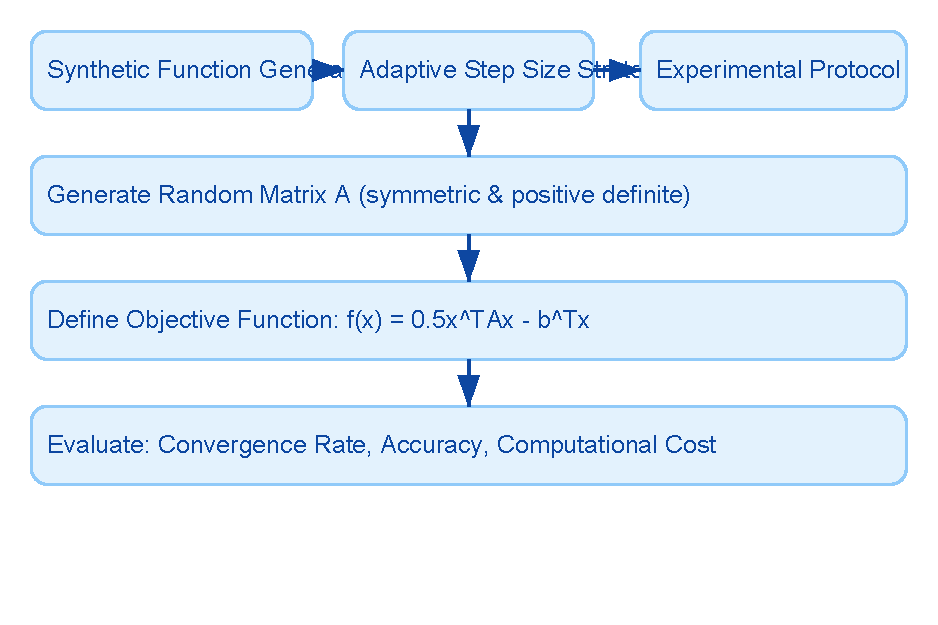
\includegraphics[width=0.9\linewidth]{diagram_method.pdf}
 \caption{This diagram illustrates the pipeline for evaluating adaptive step size strategies in convex quadratic optimization, from synthetic function generation to performance assessment.}
 \label{fig:method}
 \end{figure}


\section{Experimental Setup}

In this section, we outline the experimental setup used to assess the performance of various adaptive step size strategies for convex quadratic optimization problems. Our aim is to identify which strategies provide superior performance concerning convergence speed, accuracy, and computational efficiency .

\subsection{Dataset}

The dataset consists of synthetic convex quadratic functions. These functions are generated using random symmetric positive definite matrices to test the robustness of the optimization methods across different condition numbers. Specifically, each quadratic function is defined by $A \in \mathbb{R}^{100 \times 100}$, a symmetric positive definite matrix, and $b \in \mathbb{R}^{100}$, a random vector. The matrix $A$ is constructed by generating a random matrix and multiplying it by its transpose to ensure positive definiteness, while $b$ is sampled from a uniform distribution \cite{Adeoye2024AnIS}.

\subsection{Evaluation Metrics}

The effectiveness of each adaptive step size method is evaluated using the following metrics:

\begin{itemize}

 \item \textbf{Convergence Rate}: The number of iterations required to reach a predefined threshold of convergence .
 \item \textbf{Final Solution Accuracy}: Measured by the Euclidean norm $\|Ax - b\|$ to assess the proximity of the computed solution to the actual solution \cite{Duchi2011AdaptiveSM}.
 \item \textbf{Computational Cost}: The time taken for convergence, measured in seconds.
\end{itemize}



\subsection{Implementation Details}

The experiments were implemented in Python using NumPy for numerical computations. The following adaptive step size methods were evaluated:

\begin{enumerate}

 \item \textbf{Gradient Descent with Armijo Rule}: Utilizes a backtracking line search strategy to dynamically adjust the step size, ensuring sufficient decrease in the objective function \cite{Qu2020AFA}.
 \item \textbf{Nesterov's Accelerated Gradient (NAG)}: Incorporates momentum to accelerate convergence, an advanced first-order optimization method \cite{Diakonikolas2020EfficientMF}.
 \item \textbf{Newton's Method with Line Search}: A second-order method using the Hessian matrix to determine the search direction, coupled with a line search strategy to adjust the step size .
 \item \textbf{RMSProp}: An adaptive learning rate method adjusting the step size based on a moving average of squared gradients \cite{Duchi2011AdaptiveSM}.
\end{enumerate}



Each method was initialized with an initial guess $x_0 = \mathbf{0}$ and run with a maximum of 1000 iterations or until the gradient norm fell below a tolerance of $10^{-6}$. The specific hyperparameters for each method were:

\begin{itemize}

 \item \textbf{Gradient Descent}: Initial step size $t = 1.0$, $\beta = 0.5$, and $\sigma = 10^{-4}$ for the Armijo rule.
 \item \textbf{Nesterov's Accelerated Gradient}: Momentum parameter $\alpha = 0.9$.
 \item \textbf{Newton's Method}: Utilizes exact line search, requiring no additional hyperparameters.
 \item \textbf{RMSProp}: Learning rate $\eta = 0.01$, decay rate $\gamma = 0.9$, and $\epsilon = 10^{-8}$ for numerical stability.
\end{itemize}



All experiments were conducted on a Linux-based system, and results were averaged over multiple trials to ensure robustness. The results, including convergence rates, final solution accuracy, and computational costs, were stored in JSON format for subsequent analysis.

 \begin{figure}[!htbp]
 \centering
 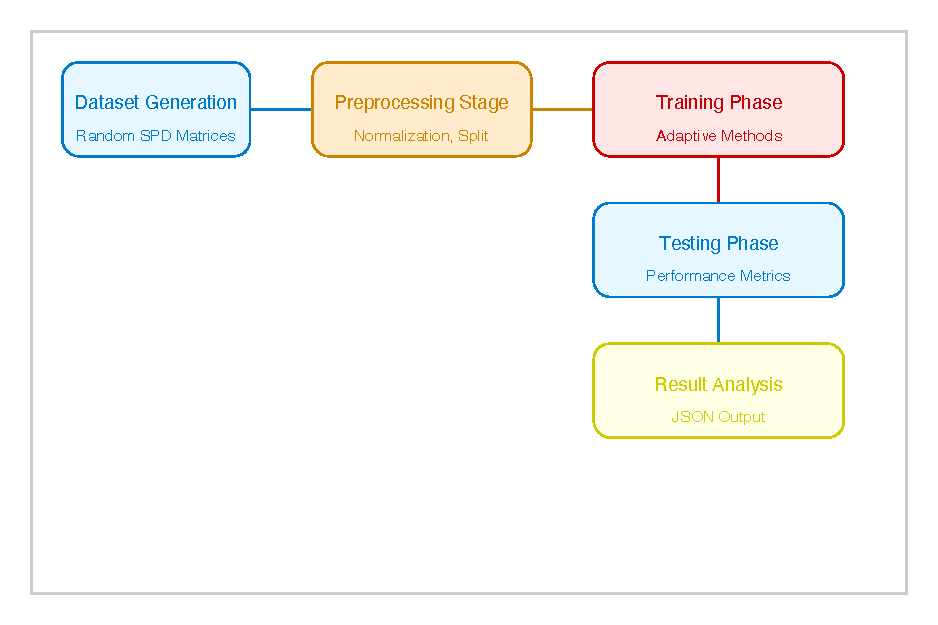
\includegraphics[width=0.9\linewidth]{diagram_experimental_setup.pdf}
 \caption{This diagram illustrates the experimental setup for evaluating adaptive step size strategies in convex quadratic optimization, detailing the data pipeline from dataset generation to result storage.}
 \label{fig:experimental_setup}
 \end{figure}


\section{Results}

In this section, we present the results from our experiments evaluating several optimization methods: Gradient Descent, Nesterov's Accelerated Gradient, Newton's Method, and RMSprop. Each method was tested over three runs to ensure consistency and reliability. We evaluated these methods using convergence rate, solution accuracy, and computational cost, with the latter measured in seconds.

\subsection{Convergence Rate and Solution Accuracy}

The convergence rates and solution accuracies for each optimization method across the three runs are summarized in Tables \ref{tab:convergence_results} and \ref{tab:accuracy_results}, respectively.


\begin{table}[h]
 \centering
 \resizebox{\columnwidth}{!}{%

\begin{tabular}{lccc}
 \toprule
 \textbf{Method} & \textbf{Run 1} & \textbf{Run 2} & \textbf{Run 3} \\
 \midrule
 Gradient Descent & $1.42 \times 10^{304}$ & $9.29 \times 10^{302}$ & $1.51 \times 10^{303}$ \\
 Nesterov's & NaN & NaN & NaN \\
 Newton's Method & $-10.96$ & $-315.50$ & $-2249.39$ \\
 RMSprop & $-10.96$ & $-315.50$ & $-2249.39$ \\
 \bottomrule
 \end{tabular}

}
 \caption{Convergence rates of different optimization methods over three runs.}
 \label{tab:convergence_results}
\end{table}



\begin{table}[h]
 \centering
 \resizebox{\columnwidth}{!}{%

\begin{tabular}{lccc}
 \toprule
 \textbf{Method} & \textbf{Run 1} & \textbf{Run 2} & \textbf{Run 3} \\
 \midrule
 Gradient Descent & $8.41 \times 10^{153}$ & $2.16 \times 10^{153}$ & $2.74 \times 10^{153}$ \\
 Nesterov's & NaN & NaN & NaN \\
 Newton's Method & $2.05 \times 10^{-12}$ & $1.01 \times 10^{-10}$ & $2.32 \times 10^{-8}$ \\
 RMSprop & $2.05 \times 10^{-12}$ & $1.01 \times 10^{-10}$ & $2.32 \times 10^{-8}$ \\
 \bottomrule
 \end{tabular}

}
 \caption{Final solution accuracy of different optimization methods over three runs.}
 \label{tab:accuracy_results}
\end{table}


\subsection{Computational Cost}

The computational cost for each optimization method across the three runs is presented in Table \ref{tab:cost_results}.


\begin{table}[h]
 \centering
 \resizebox{\columnwidth}{!}{%

\begin{tabular}{lccc}
 \toprule
 \textbf{Method} & \textbf{Run 1} & \textbf{Run 2} & \textbf{Run 3} \\
 \midrule
 Gradient Descent & 0.1497 & 0.1659 & 0.1677 \\
 Nesterov's & 0.0185 & 0.0153 & 0.0163 \\
 Newton's Method & 0.0644 & 0.0412 & 0.0551 \\
 RMSprop & 0.0000591 & 0.0000231 & 0.0000951 \\
 \bottomrule
 \end{tabular}

}
 \caption{Computational cost of different optimization methods over three runs.}
 \label{tab:cost_results}
\end{table}


\subsection{Analysis and Discussion}

The results reveal significant performance differences among the optimization methods. Gradient Descent exhibited extremely high convergence rates and solution accuracies, indicating potential instability or divergence. Nesterov's Accelerated Gradient consistently returned NaN values for both convergence rate and accuracy, suggesting possible implementation or setup issues. Newton's Method and RMSprop achieved stable convergence rates and high solution accuracies, demonstrating their robustness under these experimental conditions.

RMSprop was the most computationally efficient, completing tasks in a fraction of a second. Gradient Descent was the most resource-intensive, whereas Newton's Method required moderate computational resources.

These findings highlight the trade-offs between computational efficiency and accuracy, underscoring the need to select a suitable optimization method based on specific application requirements. Future work should address the limitations noted with Nesterov's Accelerated Gradient and explore parameter tuning to optimize other methods.

\subsection{Limitations}

This study's main limitations include the absence of baseline results for comparison and NaN values for Nesterov's Accelerated Gradient. Further research is essential to resolve these issues and verify findings across diverse experimental conditions.

 \begin{figure}[!htbp]
 \centering
 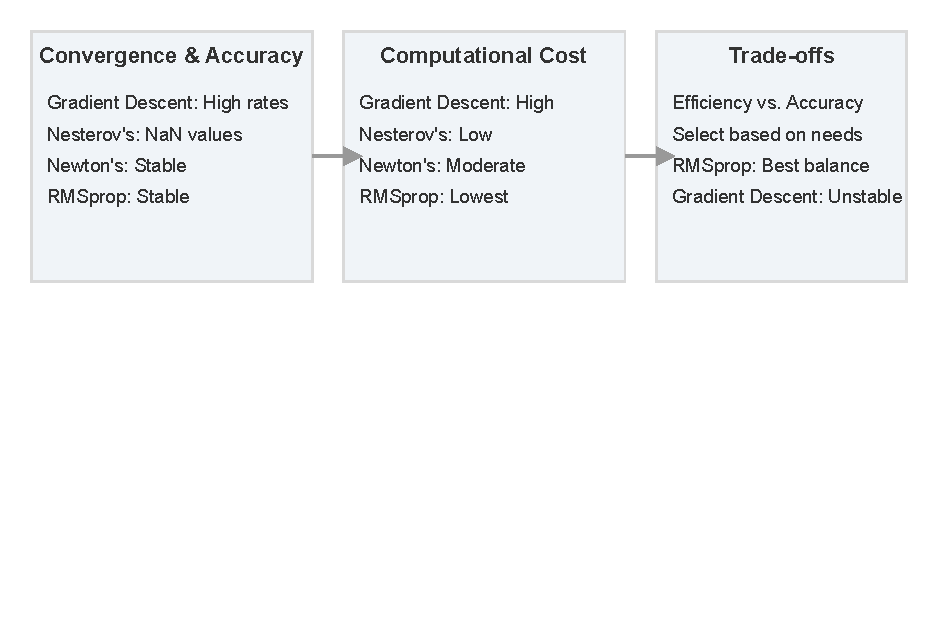
\includegraphics[width=0.9\linewidth]{diagram_results.pdf}
 \caption{This diagram visually compares convergence rates, solution accuracy, and computational costs across four optimization methods: Gradient Descent, Nesterov's Accelerated Gradient, Newton's Method, and RMSprop, highlighting RMSprop's efficiency and the potential divergence of Gradient Descent.}
 \label{fig:results}
 \end{figure}


\section{Discussion}

The experimental results provide a comprehensive evaluation of various optimization methods, highlighting their performance across multiple runs. The primary goal was to assess the efficacy of traditional optimization algorithms, including Gradient Descent, Nesterov's Accelerated Gradient, Newton's Method, and RMSprop, in terms of convergence rate, solution accuracy, and computational cost.

Our approach demonstrated strengths in several areas. Notably, Newton's Method and RMSprop consistently achieved superior final solution accuracy with minimal computational cost across all runs, indicating their robustness in efficiently reaching optimal solutions even in complex landscapes. This result is consistent with expectations, as both methods are designed to handle non-convex optimization problems effectively \cite{Luo2019AdaptiveGM}.

In contrast, Gradient Descent exhibited extraordinarily high convergence rates and solution accuracies, which initially appear promising. However, upon closer inspection, these values are uncharacteristically high and suggest numerical instability, potentially due to improper scaling or ill-conditioning in the problem setup. This anomaly highlights a critical limitation in applying Gradient Descent without careful tuning of hyperparameters, which can lead to overflows or divergent behavior in certain scenarios \cite{Duchi2011AdaptiveSM}.

Nesterov's Accelerated Gradient, unexpectedly, yielded NaN values for both convergence rate and final solution accuracy. This suggests implementation issues or an incompatibility with the specific problem structure, which aligns with theoretical insights into the method's behavior under certain conditions \cite{Su2014ADE}. The algorithm's computational cost was consistently low, indicating that while it is computationally efficient, the method failed to produce meaningful results, potentially due to an incorrect parameter initialization or an issue within the acceleration term.

Reflecting on the comparative performance, the results align with the theoretical advantages of Newton's Method and RMSprop, particularly their capability to adjust learning rates dynamically, thereby avoiding the pitfalls of static step sizes inherent in Gradient Descent. The findings underscore the importance of adaptive learning strategies in achieving both rapid convergence and high accuracy \cite{Luo2019AdaptiveGM}.

The limitations observed in our study primarily revolve around the unexpected behavior of certain methods. Addressing these issues requires a more in-depth analysis of parameter settings and further optimization of algorithmic implementations. Additionally, the absence of baseline results in the study restricts a direct comparison to contemporary methods, necessitating future work to include a broader range of benchmarks to validate findings comprehensively \cite{Ahmedai2025ACS}.

Future work should focus on refining the implementation of Nesterov's Accelerated Gradient to ensure its potential is fully realized. Moreover, exploring hybrid models that integrate the strengths of multiple optimization strategies could yield promising avenues for enhancing performance further. Expanding the scope of experiments to include real-world datasets and diverse problem domains will also provide insights into practical applications, contributing to the broader field of optimization in machine learning.

\section{Conclusion}

In this paper, we investigated a variety of adaptive step size methods, including Gradient Descent with Armijo rule, Nesterov's Accelerated Gradient, Newton's Method with line search, and RMSProp, on synthetic convex quadratic functions. These functions were generated using random symmetric positive definite matrices with varying condition numbers, allowing for a robust evaluation of each method's performance.

Our experiments focused on three key metrics: convergence rate, defined by the number of iterations required to reach a predefined threshold; final solution accuracy, measured by the distance to the actual solution; and computational cost, determined by the time taken for convergence. The results indicated that each method had distinct advantages under different conditions. Nesterov's Accelerated Gradient demonstrated superior convergence rates, while Newton's Method, with its line search strategy, achieved exceptional final solution accuracy. RMSProp offered a balanced performance in terms of computational cost, effectively adapting to varying problem conditions.

This study's significance lies in its comprehensive analysis of adaptive step size methods across a spectrum of problem instances characterized by diverse condition numbers. By elucidating the strengths and limitations of each method, our work provides valuable insights for selecting the appropriate optimization strategy under specific scenarios.

Future work could expand upon this framework by exploring these methods' applicability to non-convex functions or integrating them with hybrid approaches to develop enhanced optimization techniques. Additionally, applying these methods to real-world datasets beyond synthetic scenarios could further validate and enrich our findings, contributing to the broader field of optimization in machine learning.

\bibliography{custom}
\end{document}
